\section*{Gendererklärung}

Zur besseren Lesbarkeit werden auf dieser Website personenbezogene Bezeichnungen, die sich zugleich auf Frauen und Männer beziehen, generell nur in der im Deutschen üblichen männlichen Form angeführt, also z.B. \glqq Teilnehmer\grqq{} statt \glqq TeilnehmerInnen\grqq{} oder \glqq Teilnehmerinnen und Teilnehmer\grqq{}.

Dies soll jedoch keinesfalls eine Geschlechterdiskriminierung oder eine Verletzung des Gleichheitsgrundsatzes zum Ausdruck bringen.

\section*{Gender Declaration}

For better readability, personal names that refer to women and men at the same time are generally only given in the masculine form common in German, e.g. \glqq Participants\grqq{} instead of \glqq Participants\grqq{} or \glqq Participants\grqq{}.

However, this is in no way intended to express gender discrimination or a violation of the principle of equality.

\pagebreak

\section*{Eidesstattliche Erklärung}
Hiermit erkläre ich an Eides statt, dass ich die vorgelegte Diplomarbeit selbstständig und ohne Benutzung anderer als der angegebenen Hilfsmittel angefertigt habe. Gedanken, die aus fremden Quellen direkt oder indirekt übernommen wurden, sind als solche gekennzeichnet.

Die Arbeit wurde bisher in gleicher oder ähnlicher Weise keiner anderen Prüfungsbehörde vorgelegt und auch noch nicht veröffentlicht. \\[1em]
Leonding, am \duedatede \\[5em]
\ifthenelse{\isundefined{\firstauthor}}{}{\firstauthor}
\ifthenelse{\isundefined{\secondauthor}}{}{\kern-1ex, \secondauthor}
\ifthenelse{\isundefined{\thirdauthor}}{}{\kern-1ex, \thirdauthor}
\ifthenelse{\isundefined{\fourthauthor}}{}{\kern-1ex, \fourthauthor} \\[5em]

\section*{Declaration of Academic Honesty}
Hereby, I declare that I have composed the presented paper independently on my own and without any other resources than the ones indicated. All thoughts taken directly or indirectly from external sources are properly denoted as such.

This paper has neither been previously submitted to another authority nor has it been published yet. \\[1em]
Leonding, \duedateen \\[5em]
\ifthenelse{\isundefined{\firstauthor}}{}{\firstauthor}
\ifthenelse{\isundefined{\secondauthor}}{}{\kern-1ex, \secondauthor}
\ifthenelse{\isundefined{\thirdauthor}}{}{\kern-1ex, \thirdauthor}
\ifthenelse{\isundefined{\fourthauthor}}{}{\kern-1ex, \fourthauthor} \\[5em]

\begin{abstract}
	Die Konzentration der Schüler während des Unterrichts ist wichtig. Doch Sehr oft kommt es vor, dass in einm Klassenraum Sauerstoffmangel herrscht. Deswegen wurde von der HTBLA-Leonding ein Mesh-Netzwerk aus Mikrocontrollern in Auftrag gegeben. Dieses Mesh-Netzwerk agiert als Infrastruktur für sämtliche Sensoren und Aktoren, die in der Schule untergebracht sind und ermöglich ihnen Nachrichten untereinander zu versenden.

	Die Vorteile eines Mesh-Netzwerkes gegenüber einem normalen Wi-Fi Netzwerk sind, dass:
	\begin{itemize}
		\item jeder Mikrocontroller wieder einen eigenen Access Point öffnet und somit das Mesh-Netzwerk an größere Reichweite gelangt
		\item ein Mesh-Netzwerk auf ausfallende Knoten selbständig reagieren kann und die Netzwerkstruktur automatisch anpasst
		\item Mesh-Netzwerke leicht skalierbar sind, da um die Reichweite des Netzwerkes anzupassen nur Mikrocontroller hinzugefügt oder entfernt werden müssen
		\item der Benutzer sich nicht darum kümmern muss mit welchem Knoten er sich verbindet. Vom Standpunkt des Benutzers sehen die verschiedenen Accesspoints der Mikrocontroller wie ein großes Wi-Fi Netzwerk aus.
	\end{itemize}
	\begin{figure}[H]
        \begin{center}
            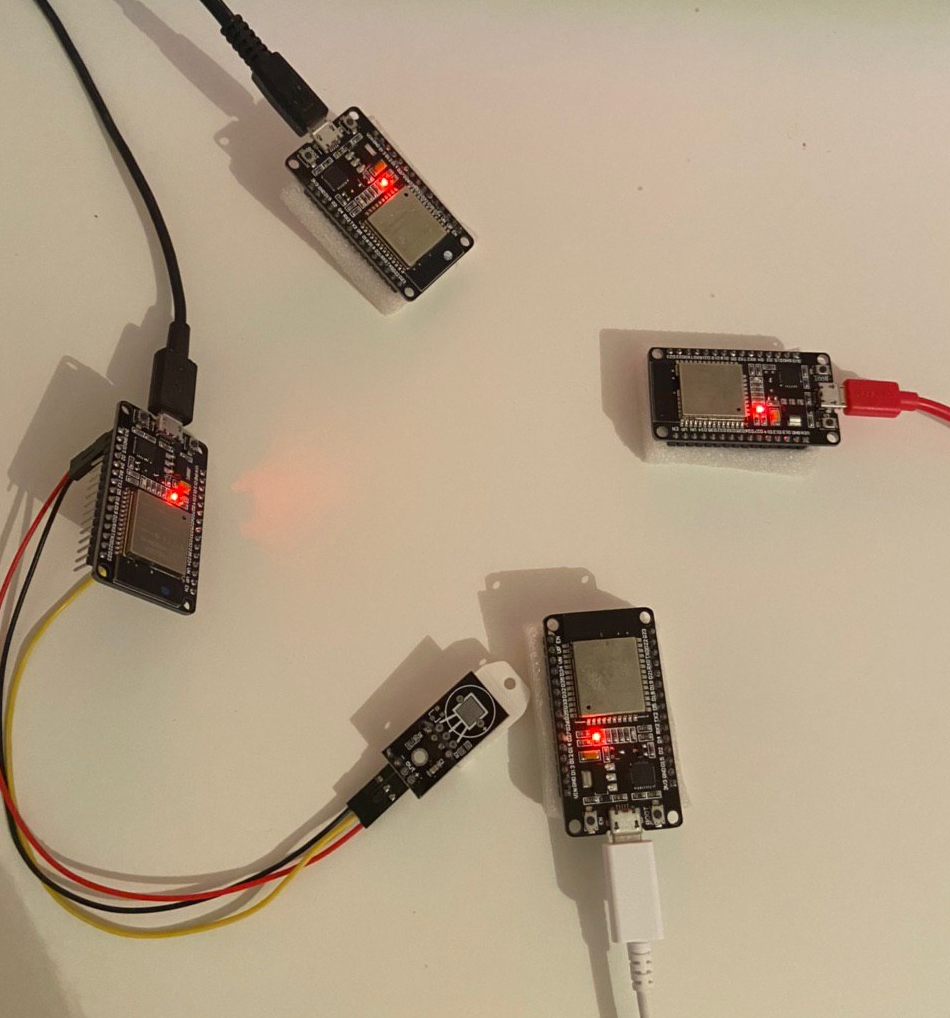
\includegraphics[scale=0.31]{images/meshnetwork-esp32.png}
            \caption{Mikrocontroller in einem Meshnetzwerk (Quelle: eigene Darstellung)}
        \end{center}
    \end{figure}
\end{abstract}

\begin{otherlanguage}{english}
\begin{abstract}
	
	The concentration of the students during class is very important. But often it happens that there is a lack of oxygen in a classroom. That is why the HTBLA-Leonding commissioned a mesh network of microcontrollers to be designed. This mesh network acts as an infrastructure for all sensors and actuators in the school and enables them to send messages to one another.

	The advantages of a mesh network over a normal Wi-Fi network are the following:
	\begin{itemize}
		\item each microcontroller opens its own access point thus making the mesh network reache a greater range
		\item a mesh network can react independently to failing nodes and automatically adjusts the network structure
		\item Mesh networks are easily scalable, to adjust the range of the network only microcontrollers have to be added or removed
		\item the user does not have to worry about which node to connect to. From the user's point of view, the various access points of the microcontrollers look like a large Wi-Fi network.
	\end{itemize}
	\begin{figure}[H]
        \begin{center}
            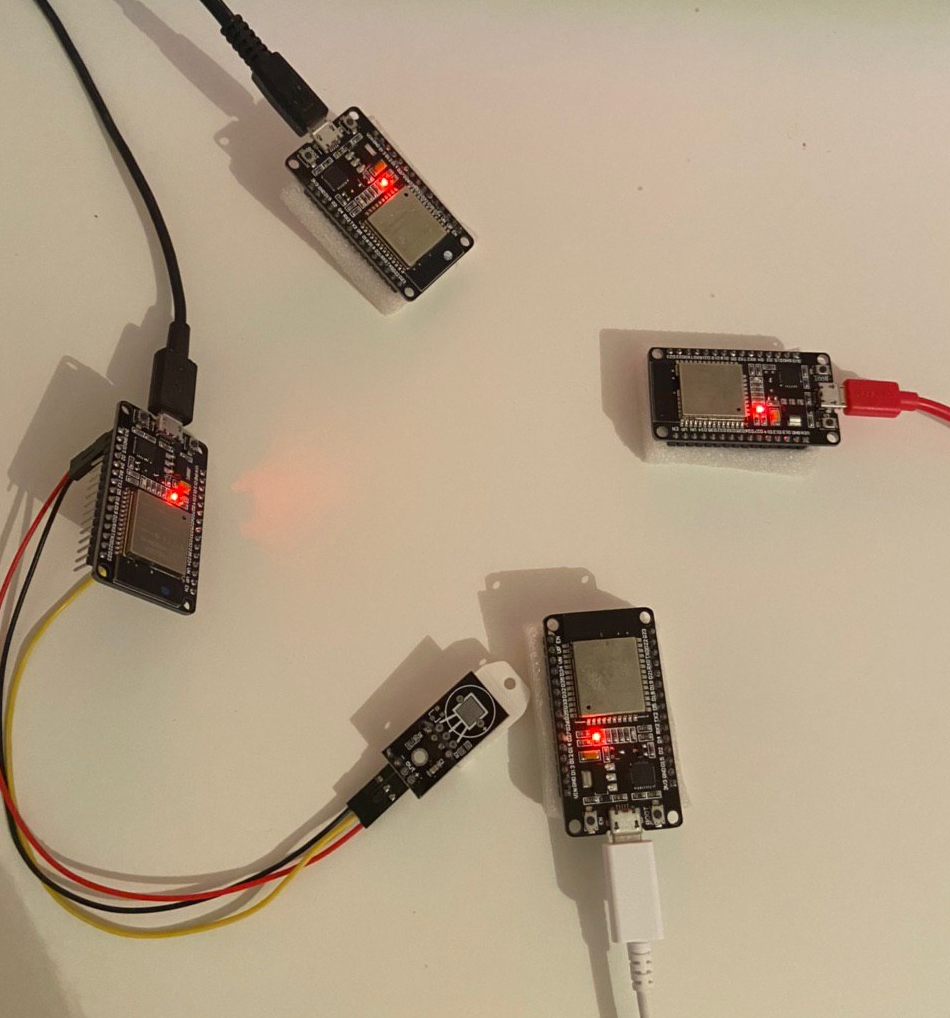
\includegraphics[scale=0.31]{images/meshnetwork-esp32.png}
            \caption{microcontroller in a meshnetwork (source: own source)}
        \end{center}
    \end{figure}
\end{abstract}
\end{otherlanguage}


\section*{Autoren der Diplomarbeit}
\subsection*{Tim Untersberger}
\subsubsection*{Aufgabenbereich}
% TODO: write
\begin{figure}[H]
	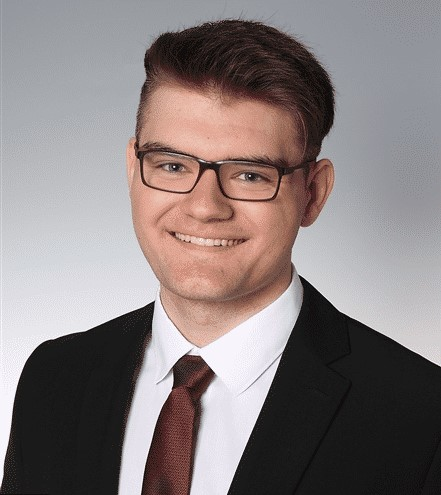
\includegraphics[scale=0.3]{images/tim_untersberger.jpg}
\end{figure}
\begin{table}[htb]
\begin{tabular}{ll}
Name:                            & Tim Untersberger          \\
Geburtsdatum:                    & 15. April 2001                   \\
E-Mail:                          & timuntersberger2@gmail.com          \\
                                 &                               \\
\textbf{Bildungsweg:}            &                               \\  
2007 bis 2011                    & Volksschule Doppl          \\
2011 bis 2015                    & NMS Hart     \\
seit 2015                        & HTL Leonding, Informatik      \\
                                 &                               \\
\textbf{Berufliche Erfahrung:}   &                               \\
Sommer 2016                      & {Colour \& Point}, Softwareentwickler \\
Sommer 2018                      & Runtastic, Softwareentwickler \\
                                 &                               \\
\textbf{Sprachliche Kenntnisse:} &                               \\
Deutsch                          & Muttersprache                 \\
Englisch                         & Fließend                     
\end{tabular}
\end{table}
\pagebreak
\subsection*{Stefan Waldl}
\subsubsection*{Aufgabenbereich}
\begin{figure}[H]
	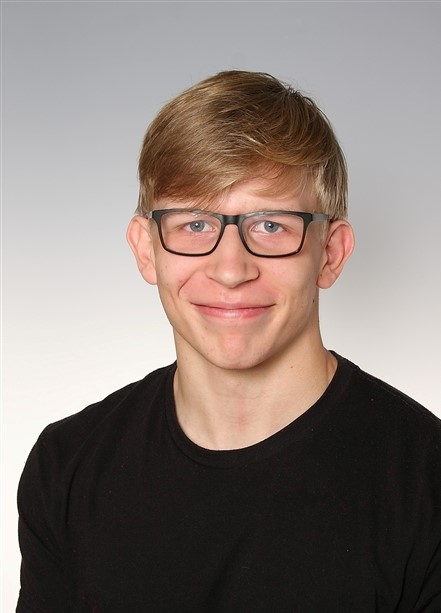
\includegraphics[scale=1]{images/stefan_waldl.jpg}
\end{figure}
\begin{table}[htb]
\begin{tabular}{ll}
Name:                            & Tim Untersberger          \\
Geburtsdatum:                    & 15. April 2001                   \\
E-Mail:                          & timuntersberger2@gmail.com          \\
                                 &                               \\
\textbf{Bildungsweg:}            &                               \\  
2007 bis 2011                    & Volksschule Doppl          \\
2011 bis 2015                    & NMS Hart     \\
seit 2015                        & HTL Leonding, Informatik      \\
                                 &                               \\
\textbf{Berufliche Erfahrung:}   &                               \\
Sommer 2016                      & {Colour \& Point}, Softwareentwickler \\
Sommer 2018                      & Runtastic, Softwareentwickler \\
                                 &                               \\
\textbf{Sprachliche Kenntnisse:} &                               \\
Deutsch                          & Muttersprache                 \\
Englisch                         & Fließend                     
\end{tabular}
\end{table}
\pagebreak
 

\section*{Danksagung}

An dieser Stelle möchten wir uns bei all denjenigen bedanken, die uns während der
Planung und Durchführung dieser Diplomarbeit unterstützt und motiviert haben.

Ganz besonderen Dank an Herrn Prof. Thomas Stütz und Herrn Prof. Gerald Köck, welche uns bereits sehr früh unterstützt haben und unser Augenmerk auf die richtigen Technologien gelenkt haben, sowie uns auch betreut und unsere Arbeit begutachtet haben.

Bedanken wollen wir uns auch bei all unseren KorrekturleserInnen der Dokumente, welche
uns für eine fehlerfreie und ordentliche Einreichung beiseite standen.